    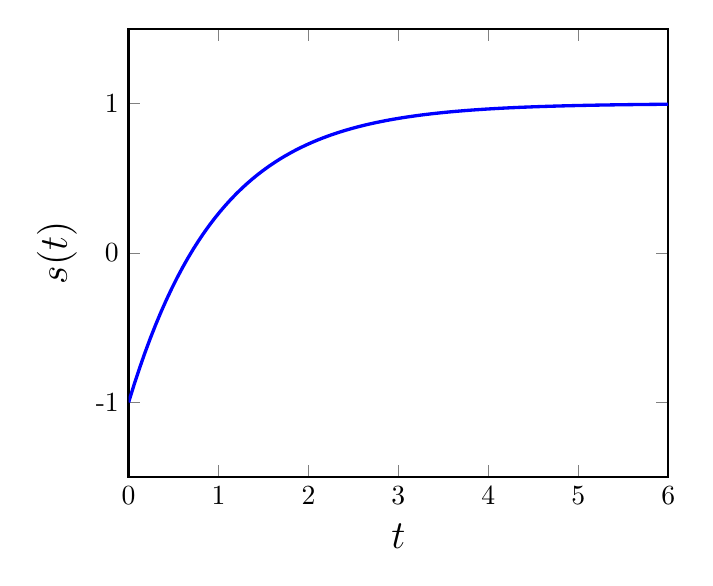
\begin{tikzpicture}%[baseline=0]
        \begin{axis}[
        scaled y ticks = false,
        axis line style = thick,
        %height=5cm,
        %width=9cm,
        %axis x line=center,
        %axis y line=center,
        xmin=0,
        xmax=6.0,
        ymin=-1.5,
        ymax=1.5,
        xlabel={$t$},
        ylabel={$s(t)$},
        %xlabel style={below right},
        %ylabel style={above left},
        yticklabels={-1,0,1},
        ytick={-1,0,1.0},
        y tick label style={anchor=east},
        label style={font=\Large},
        ]
        \addplot [very thick,color=blue,domain=0:6, samples=101]{1-2*exp(-x)};
        \end{axis}
    \end{tikzpicture}
